\documentclass[UTF8,a4paper]{paper}
\usepackage{ctex}
\usepackage[utf8]{inputenc}
\usepackage{amsmath}
\usepackage{amssymb}
\usepackage{pdfpages}
\usepackage{graphicx}
\usepackage{xcolor}
\title{模式识别作业9}
\author{张蔚桐\ 2015011493\ 自55}
\begin {document}
\maketitle
\section{学习方法的选择}
首先我们实验了线性分类方法,得到在一维情况下的概率密度函数如图\ref{1}所示,
可以看出存在着明显的交叠现象。之后采用了SVM,Adaboost,决策树,kNN等方法,
发现准确率均在92\%以下。其中SVM在92\%左右,其中线性SVM分类性能可超过90\%,
SVM之外的其他方法均没有实用价值。

之后我们采取了对神经网络的训练,发现神经网络在训练初始化条件理想的情况下可以达到
93\%以上,先后采取了5,10,20,40,80,100,200隐节点数量进行了测试,发现80隐节点时
训练速度和正确率均较好,其中过少的节点训练正确率比较低,而过多的节点不仅训练速度偏慢,
而且过拟合现象严重。因此我们选择使用80节点神经网络作为学习方法。

\begin{figure}[h]\centering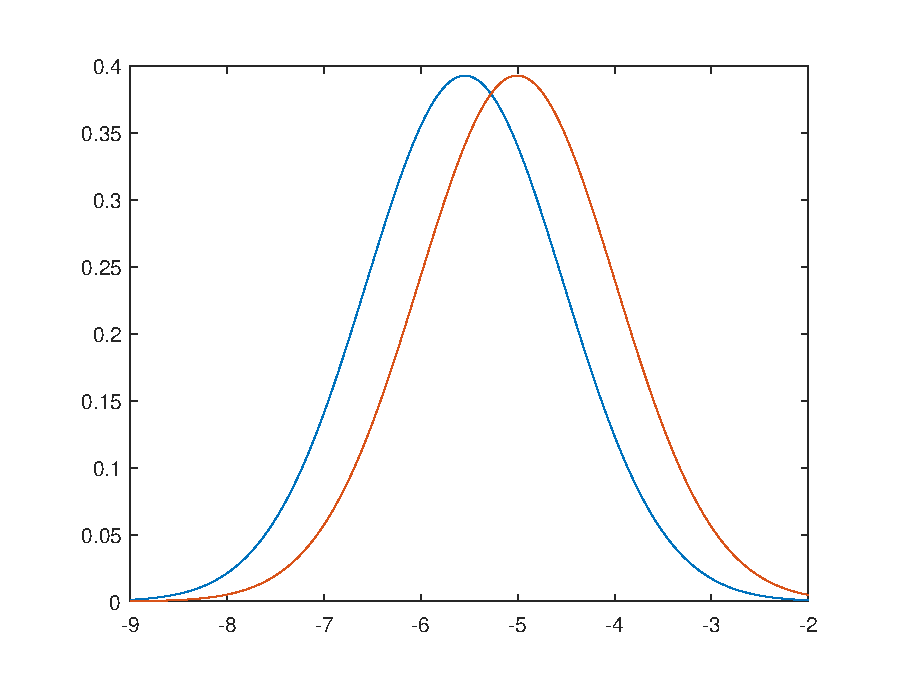
\includegraphics[width=\textwidth]{fisher.eps}
\caption{fisher方法+窗函数方法确定的一维概率密度函数}\label{1}\end{figure}

\section{特征选取方法}
已经学习的特征选择和提取方法包括遗传算法,前向后向方法,PCA,KL变换(对于二分类问题相当于Fisher方法)
等方法,其中t-SNE,LLE方法一般仅用来进行平面显示。我们尝试了遗传算法,采用神经网络的测试错误率作为
最小化目标,经过长时间计算发现错误率仅能降低到7\%,完全在神经网络的训练波动范围内。因此包括前向后向,
遗传算法等特征选择方法无效。

采用PCA方法对数据集99\%的方差进行识别之后,发现训练正确率出现了明显的下降,考虑是因为整个训练集的方差
方向和类间方差的方向不一致导致核心特征不被选择,或存在明显的非线性导致的。因此特征提取算法无效。

因此不对训练样本进行任何形式的特征提取。

\section{训练过程}
首先我们对神经网络采取了两种训练方式,如下所示
\begin{itemize}
\item 量化共轭梯度法(trainscg)

对应采取了交叉熵作为误差函数,这种方法训练速度比较快,资源占用比较小

\item 贝叶斯规则(trainbr)

对应采取了最小误差(MSE)作为误差函数,这种方法训练速度比较慢,但是可能得到更好的结果。
\end{itemize}

为避免训练波动引起的误差,我们连续训练100次,取测试集上表现最好的一组模型来预测给定的数据。
训练流程图如图\ref{2}所示。

\begin{figure}[b]\centering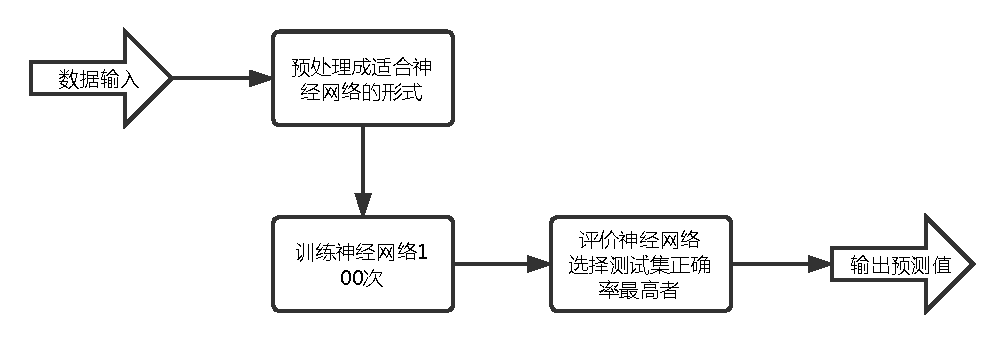
\includegraphics[width=\textwidth]{flow.pdf}
\caption{训练流程图}\label{2}\end{figure}

\section{估计预测准确率}
估计预测准确率在93\%左右。
\section{程序代码}
程序代码随附件上交,其中$train\_network.m$中$scg$变量为描述使用训练方法的变量,$scg = 1$时按照量化共轭梯度法迭代权值,$scg = 0$时按照贝叶斯规则迭代权值。
\end{document}